%************************************************
\chapter{RAFFT: Efficient prediction of fast-folding pathways of RNAs}\label{ch:rafft}
%************************************************

We propose a novel heuristic to predict RNA secondary structures. The algorithm is inspired by the kinetic partitioning mechanism, by which molecules follow alternative folding pathways to their native structure, some much faster than others. Similarly, our algorithm \texttt{RAFFT} generates an ensemble of concurrent folding pathways ending in multiple metastable structures for each given sequence; this is in contrast with traditional thermodynamic approaches, that find single structures with minimal free energies. When analyzing $50$ predicted folds per sequence, we found near-native predictions for RNAs of length $\leq 200$ nucleotides, matching the performance of recent deep-learning-based structure prediction methods. Our algorithm also acts as a folding kinetic ansatz, which we tested on two RNAs: the coronavirus frameshifting stimulation element (CFSE) and a classic bi-stable sequence. For the CFSE, an ensemble of $68$ distinct structures computed by \texttt{RAFFT} allowed us to produce complete folding kinetic trajectories, whereas known methods require evaluating millions of sub-optimal structures to achieve this result. For the second application, only $46$ distinct structures were required to reproduce the kinetics, whereas known methods required a sample of $20,000$ structures. Thanks to he fast Fourier transform on which \texttt{RAFFT} is based, these computations are efficient, with complexity $\mathcal{O}(L^2 \log L)$. 

\section*{Material and Methods}
\subsection*{Folding algorithm}
We now describe the folding algorithm starting from a sequence of nucleotides \(S=(S_1\dots S_L)\) of length \(L\), and its associated unfolded structure. We first create a numerical representation of \(S\) where each nucleotide is replaced by a unit vector of $4$ components:
\begin{equation}
\begin{split}
A \rightarrow \begin{pmatrix} 1\\ 0\\ 0\\ 0 \end{pmatrix},
U \rightarrow \begin{pmatrix} 0\\ 0\\ 0\\ 1 \end{pmatrix},
C \rightarrow \begin{pmatrix} 0\\ 1\\ 0\\ 0 \end{pmatrix},
G \rightarrow \begin{pmatrix} 0\\ 0\\ 1\\ 0 \end{pmatrix}.
\end{split}
\end{equation}
This encoding gives us a (\(4 \times L\))-matrix we call \(X\), where each row corresponds to a nucleotide as shown below:
\begin{equation}
X = \begin{pmatrix} X^A\\ X^C\\ X^G\\ X^U \end{pmatrix} = \begin{pmatrix} X^A(1) &X^A(2) &\dots &X^A(L) \\ X^C(1) &X^C(2) &\dots &X^C(L)\\ X^G(1) &X^G(2) &\dots &X^G(L)\\ X^U(1) &X^U(2) &\dots &X^U(L) \end{pmatrix}
\end{equation}
For example, \(X^A(i) = 1\) if \(S_i = A\). Next, we create a second copy \(\bar{S}=(\bar{S_L}\dots \bar{S_1})\) for which we reversed the sequence order. Then, each nucleotide of \(\bar{S}\) is replaced by one of the following unit vectors:
\begin{equation}
\begin{split}
\bar{A} \rightarrow \begin{pmatrix} 0\\ 0\\ 0\\ w_{\scalebox{0.5}{AU}}\\ \end{pmatrix},
\bar{U} \rightarrow \begin{pmatrix} w_{\scalebox{0.5}{AU}}\\ w_{\scalebox{0.5}{GU}}\\ 0\\ 0\\ \end{pmatrix},
\bar{C} \rightarrow \begin{pmatrix} 0\\ 0\\ w_{\scalebox{0.5}{GC}}\\ 0\\ \end{pmatrix},
\bar{G} \rightarrow \begin{pmatrix} 0\\ w_{\scalebox{0.5}{GC}}\\ 0\\ w_{\scalebox{0.5}{GU}}\\ \end{pmatrix}.
\end{split}
\end{equation}
\(\bar{A}\) (respectively \(\bar{U}, \bar{C}, \bar{G}\)) is the complementary of \(A\) (respectively \(U, C, G\)). \(w_{AU}\), \(w_{GC}\), \(w_{GU}\) represent the weights associated with each canonical base pair, and they are chosen empirically. We call this complementary copy \(\bar{X}\), the mirror of \(X\).

\begin{figure}[t!]
	\centering
	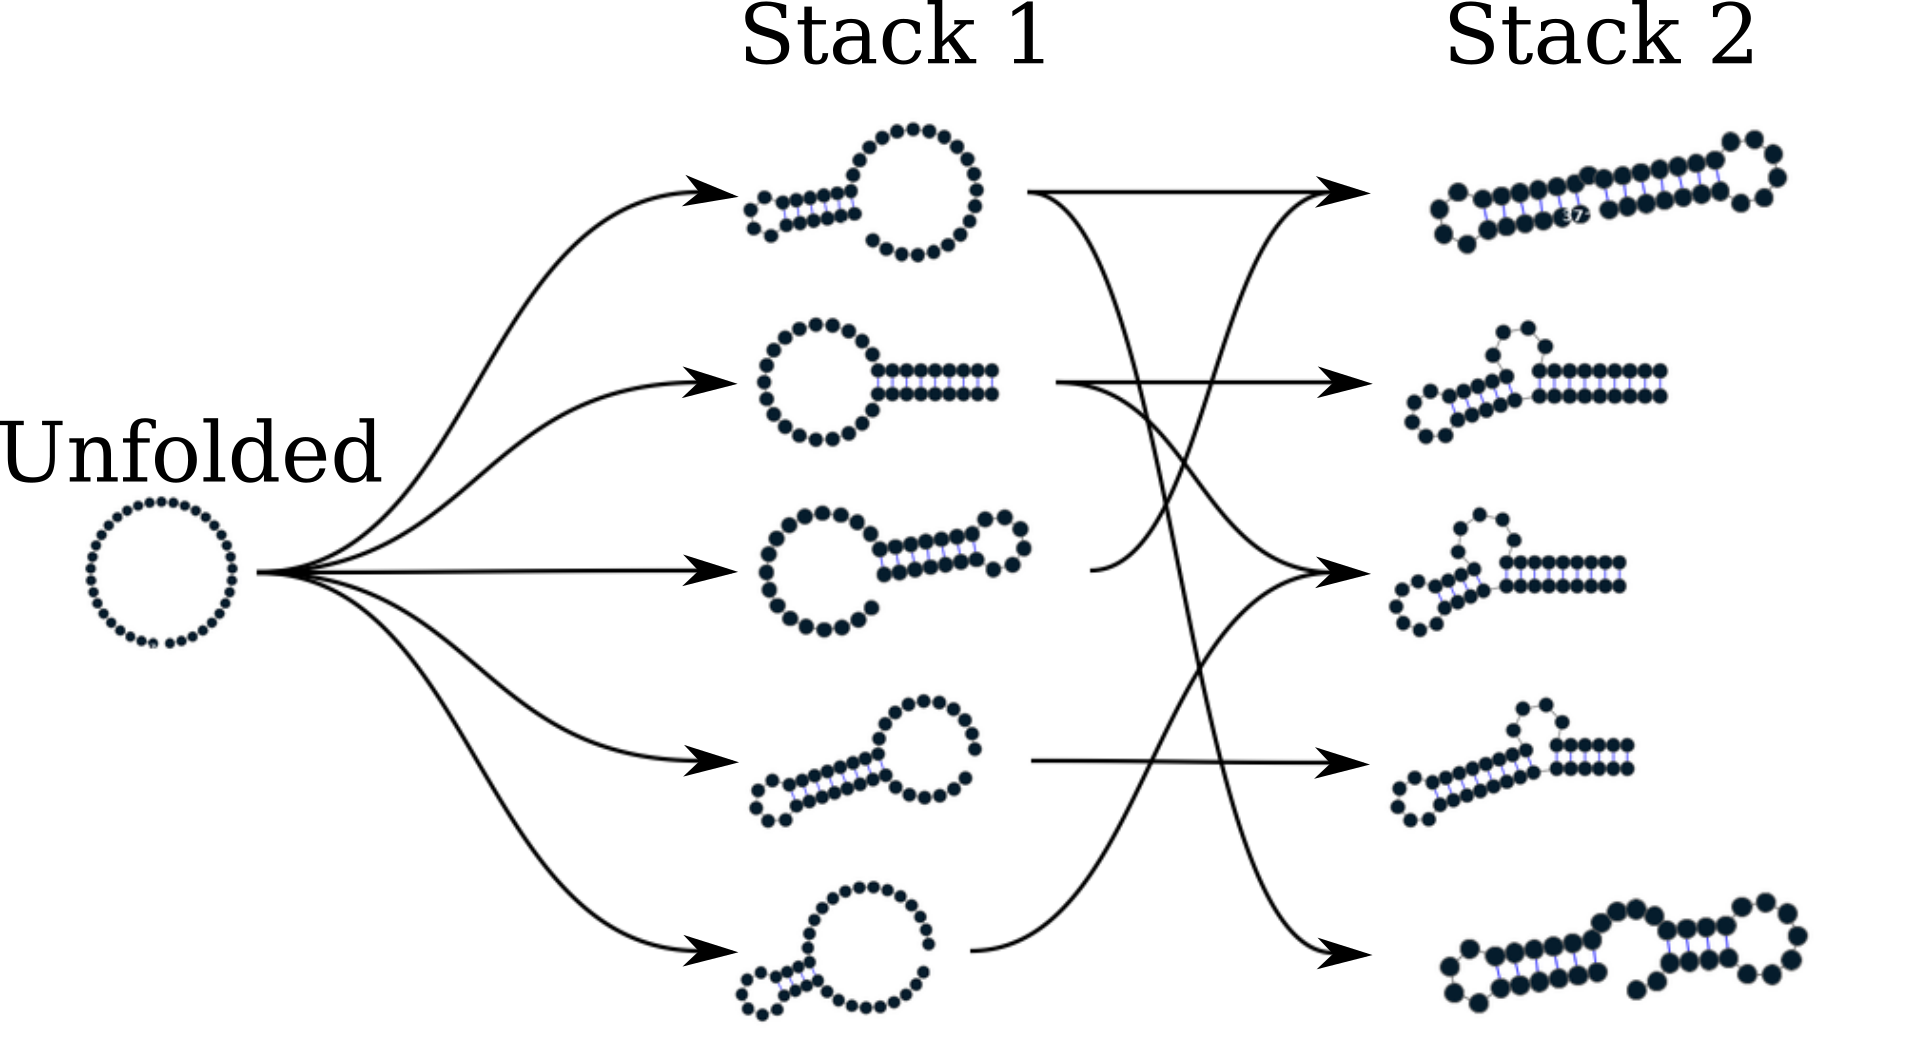
\includegraphics[width=1\linewidth]{../res/images/rafft/fast_paths_graph.png}
	\caption{\label{fast_path_graph}\textbf{Fast folding graph constructed using \texttt{RAFFT}.} In this example, the sequence is folded in two steps. The algorithm starts with the unfolded structure on the left. The \(N=5\) best stems are stored in stack 1. From stack 1, multiple stems formation are considered, but only the \(N=5\) best are stored in stack 2. Structures are ordered (from top to bottom) by energy in each stack. All secondary structure visualizations were obtained using \texttt{VARNA} \cite{darty09_varna}.}
\end{figure}


\begin{figure*}[t!]
	\centering
	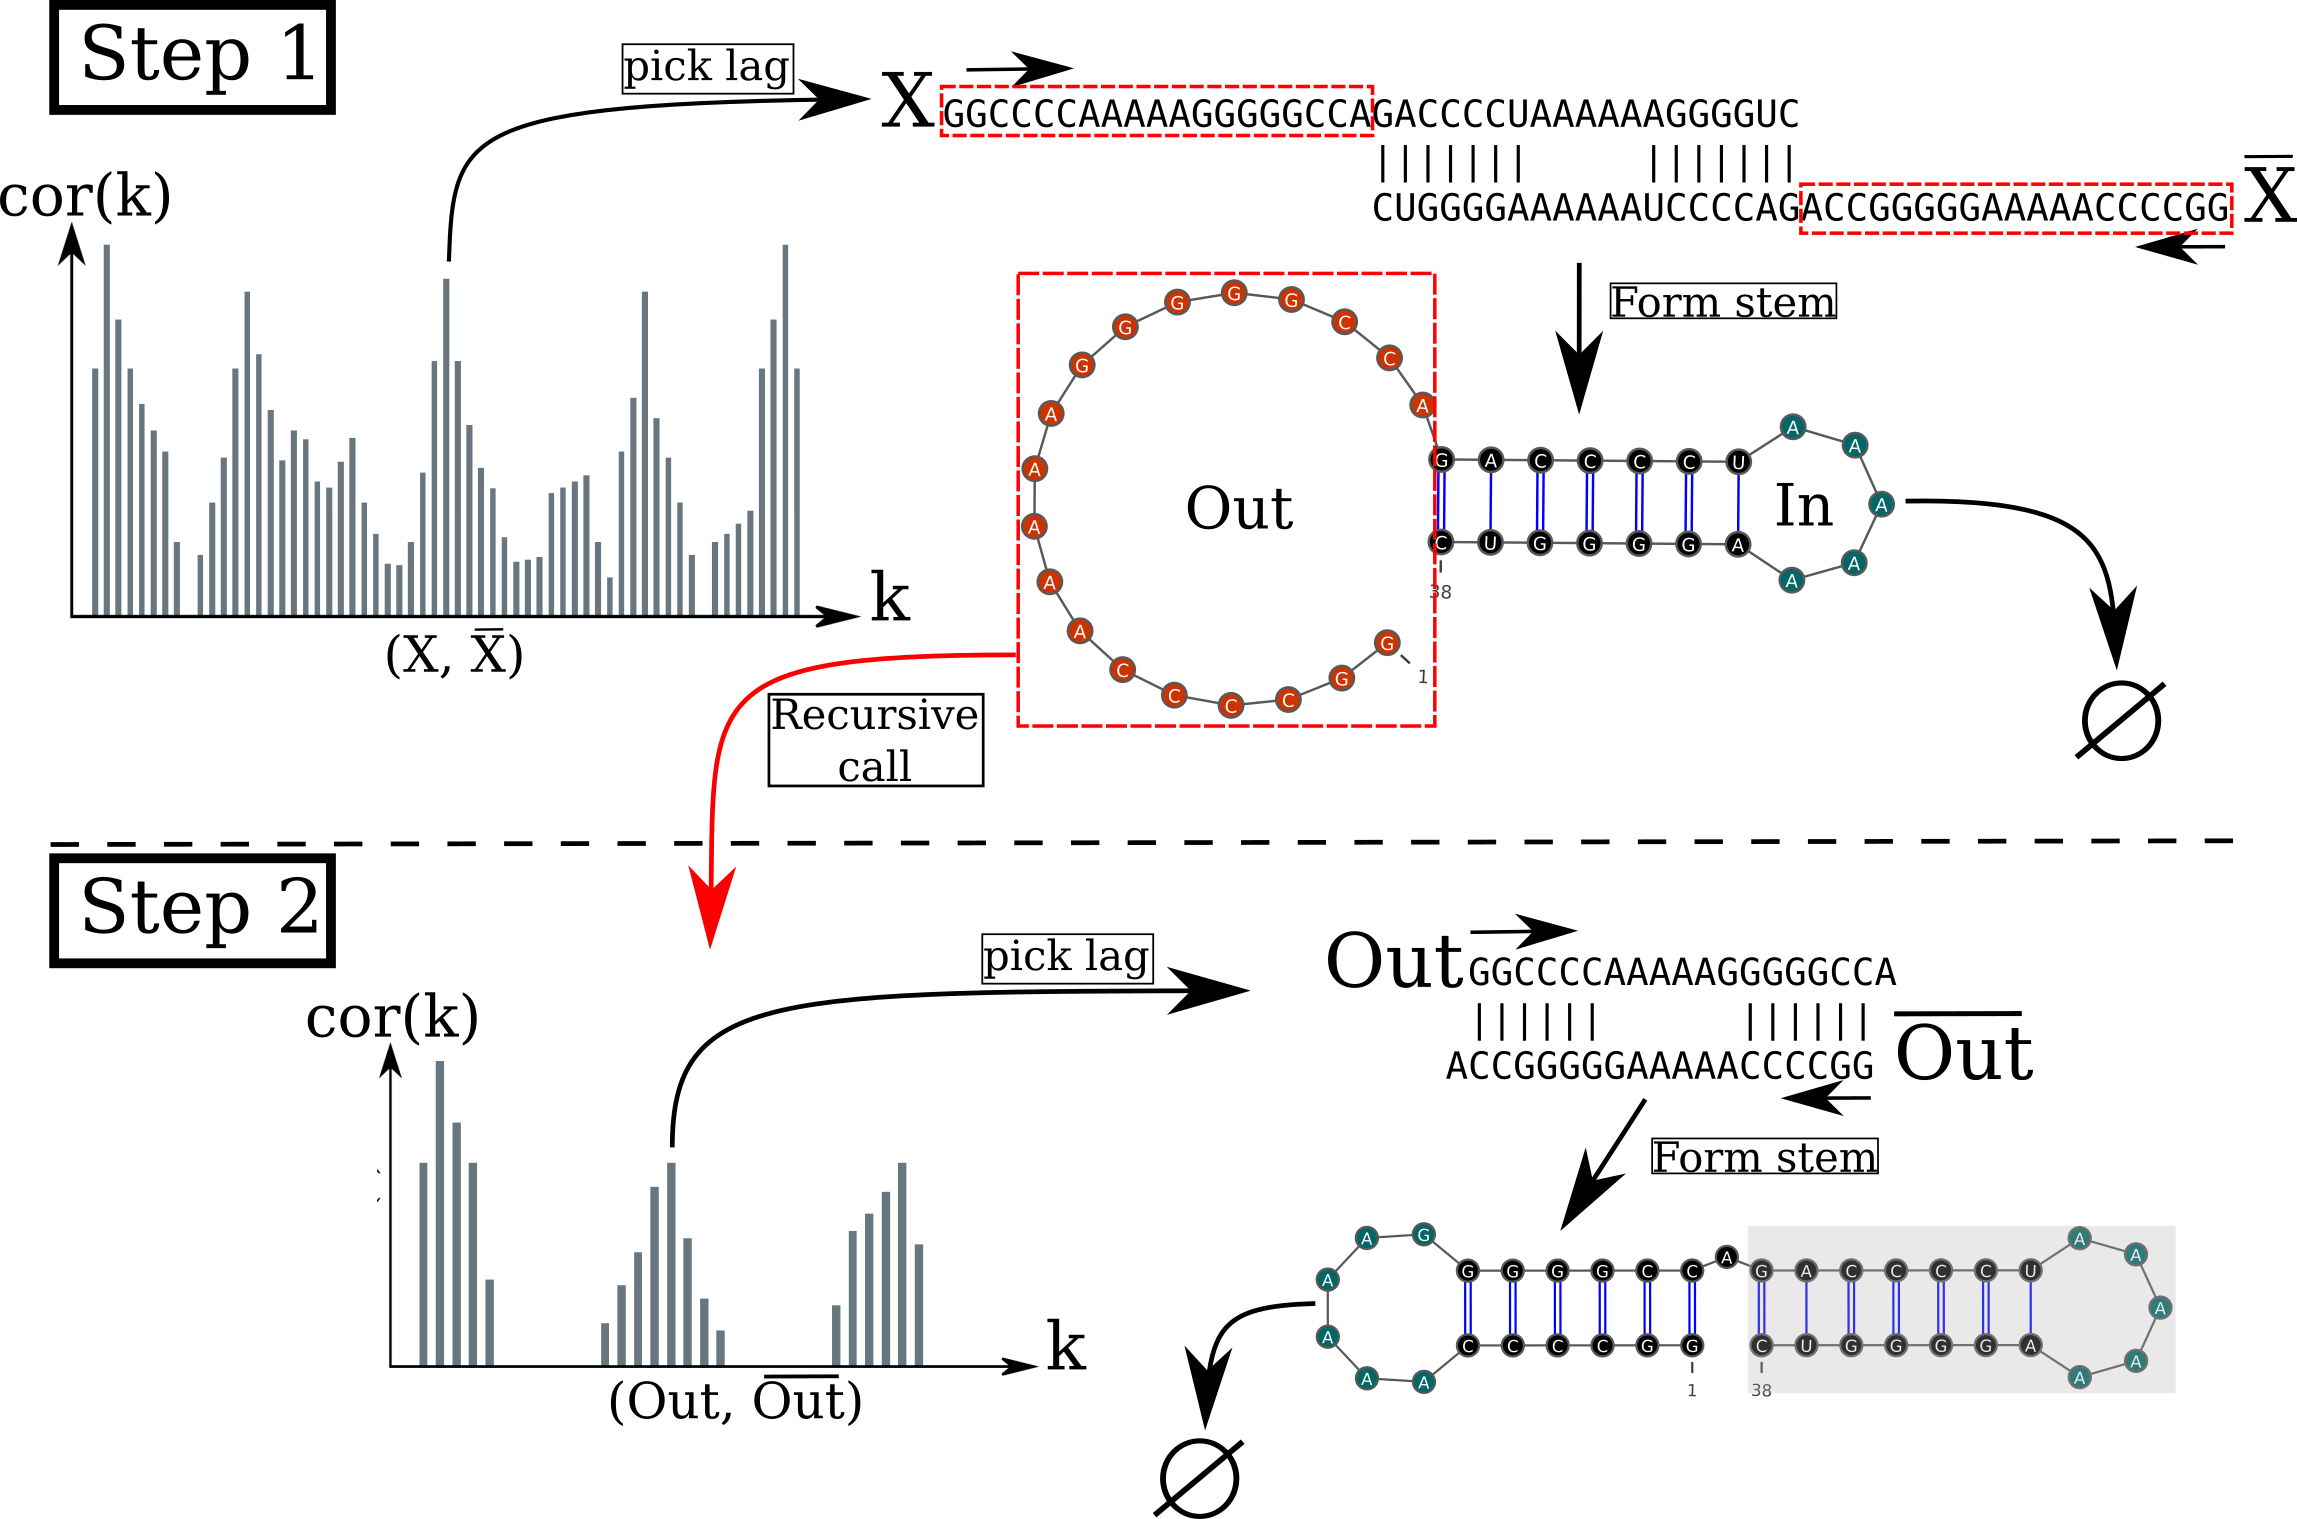
\includegraphics[width=.7\linewidth]{../res/images/rafft/algo_draw.png}
	\caption{\label{algo_desc}\textbf{Algorithm execution for one example sequence which requires two steps.} (Step 1) From the correlation $cor(k)$, we select one peak which corresponds to a position lag $k$. Then, we search for the largest stem and form it. Two fragments, ``In" (the interior part of the stem) and ``Out" (the exterior part of the stem), are left, but only the ``Out" may contain a new stem to add. (Step 2) The procedure is called recursively on the ``Out" sequence fragment only. The correlation $cor(k)$ between the ``Out'' fragment and its mirror is then computed and analyzing the $k$ positional lags allows to form a new stem. Finally, no more stem can be formed on the fragment left (colored in blue), so the procedure stops.}
\end{figure*}


To search for stems, we use the complementary relation between \(X\) and \(\bar{X}\) with the correlation function \(\text{cor}(k)\). This correlation is defined as the sum of individual \(X\) and \(\bar{X}\) row correlations:
\begin{equation}
\text{cor}(k)=\sum_{\alpha \in \{A,U,C,G\}}c_{X^{\alpha},\bar{X}^{\alpha}}(k),
\end{equation}
where a row correlation between \(X\) and \(\bar{X}\) is given by:
\begin{equation}
c_{X^\alpha,\bar{X}^\alpha}(k) = \sum\limits_{\substack{1\leq i \leq L\\1 \leq i + k \leq L}} \frac{X^\alpha(i) \bar{X}^\alpha(i+k)}{\text{min}(k, 2 L-k)}.
\end{equation}
For each \(\alpha \in \{A,U,C,G\}\), \(X^\alpha(i) \times \bar{X}^\alpha(i+k)\) is non zero if sites \(i\) and \(i+k\) can form a base pair, and will have the value of the chosen weight as described above. If all the weights are set to $1$, \(\text{cor}(k)\) gives the frequency of base pairs for a positional lag \(k\). Although the correlation naively requires \(O(L^2)\) operations, it can take advantage of the FFT which reduces its complexity to \(\mathcal{O}(L\;\text{log}(L))\).

Large \(\text{cor}(k)\) values between the two copies indicate positional lags \(k\) where the frequency of base pairs is likely to be high. However, this does not allow to determine the exact stem positions. Hence, we use a sliding window strategy to search for the largest stem within the positional lag (since the copies are symmetrical, we only need to slide over one-half of the positional lag). Once the largest stem is identified, we compute the free energy change associated with the formation of that stem. Next, we perform the same search for the \(n\) highest correlation values, which gives us \(n\) potential stems. Then, we define as the current structure the stem with the lowest free energy. Here, free energies were computed using Turner2004 energy parameters through ViennaRNA package API \cite{lorenz11_vienn_packag}.

We are now left with two independent parts, the interior and the exterior of the newly formed stem. If the exterior part is composed of two fragments, they are concatenated into one. Then, we apply recursively the same procedure on the two parts independently in a ``Breadth-First" fashion to form new consecutive base pairs. The procedure stops when no base pair formation can improve the energy. When multiple stems can be formed in these independent fragments, we combine all of them and pick the composition with the best overall stability. If too many compositions can be formed, we restrict this to the $10^4$ bests in terms of energy. Figure \ref{algo_desc} shows an example of execution to illustrate the procedure. 

The complexity of this algorithm depends on the number and size of the stems formed. The main operations performed for each stem formed are: (1) the evaluation of the correlation function \(\text{cor}(k)\), (2) the sliding-window search for stems, and (3) the energy evaluation. We based our approximate complexity on the correlation evaluation since it is the more computationally demanding step; the other operations only contribute a multiplicative constant at most. The best case is the trivial structure composed of one large stem where the algorithm stops after evaluating the correlation on the complete sequence. At the other extreme, the worst case is one where at most \(L/2\) stems of size $1$ (exactly one base pair peer stems) can be formed. The approximate complexity therefore depends on \(\sum_{i=0}^{L/2} (L-2i) \log(L-2i) \ = \mathcal{O}(L^2\log{L})\). Figure \ref{comp_plot} plots the execution time of a naive implementation of \texttt{RAFFT} and that of \texttt{RNAfold} for $20$ random sequences of various lengths, showing a substantial speed-up for larger sequences. 

The algorithm described so far tends to be stuck in the first local minima found along the folding trajectory. To alleviate this, we implemented a stacking procedure where the \(N\) best trajectories are stored in a stack and evolved in parallel. Figure \ref{fast_path_graph} illustrates this modified procedure. Like the initial version, the algorithm starts with the unfolded structure; then, the \(N=5\) best potential stems are stored in the first stack. From these \(N\) structures, the procedure tries to add stems in the unpaired regions left and saves the \(N\) best structures formed. Once no stem can be formed, the algorithm stops and output the structure with the best energy found among the structures stored in the last stack. This algorithm leads to the construction of a graph we call a \emph{fast-folding graph}. In this graph, two structures are connected if the transition from one to another corresponds to the formation of a stem or if the two structures are identical.

\begin{table*}[htbp]
	\caption{\label{average_perf}\textbf{Average performance displayed in terms of PPV and sensitivity.} The metrics were first averaged at fixed sequence length, limiting the over-representation of shorter sequences. The first two rows show the average performance for all the sequences for each method. The bottom two rows correspond to the performances for the sequences of length \(\leq\) $200$ nucleotides. For the ML and MFE only one prediction per sequence and for \texttt{RAFFT} $50$ predictions per sequence were used. Here \texttt{RAFFT} (respectively \texttt{RAFFT}*) refers to the case when the lowest free energy (resp. highest PPV) out of the $50$ predictions is selected.}
	\centering
	\begin{tabular}{lrrrr}
		\hline
		& \texttt{RAFFT} & \texttt{RAFFT}* & MFE  & ML\\
		\hline
		& \multicolumn{4}{c}{All sequences}\\
		\cmidrule{2-5}
		PPV         & 47.7  & 60.0   & 55.9 & 70.4\\
		Sensitivity & 52.8  & 62.8   & 63.3 & 77.1\\
		\hline
		& \multicolumn{4}{c}{Sequences with lengths \(\leq 200\)}\\
		\cmidrule{2-5}
		PPV         & 57.9  & 79.4   & 59.5 & 76.7\\
		Sensitivity & 63.2  & 81.2   & 65.5 & 82.9\\
		\hline
	\end{tabular}
\end{table*}

\subsection*{Kinetic ansatz}
The folding kinetic ansatz used here is derived from the fast-folding graph and allows us to model the slow processes in RNA folding. As described in Figure \ref{fast_path_graph}, transitions can occur from left to right (and right to left) but not vertically. The fast-folding graph follows the idea that parallel pathways quickly reach their endpoints; however, when the endpoints are non-native states, this ansatz allows slowly folding back into the native state \cite{pan97_foldin_rna_invol_paral_pathw}. 

As usually done, the kinetics is modelled as a continuous-time Markov chain \cite{lorenz20_effic_comput_base_probab_multi_rna_foldin}, where populations of structure evolve according to transition rates. In this context, an Arrhenius formulation is commonly used to derive transition rates \(r(x \rightarrow y) \propto \text{exp}(-\beta E^{\ddagger})\), where \(E^{\ddagger}\) is the activation energy separating \(x\) from \(y\), and \(\beta\) is the inverse thermal energy (mol/kcal). In contrast, our kinetic ansatz uses transition rates \(r(x\rightarrow y)\) based on the Metropolis scheme already used in \cite{klemm2008funnels}, and defined as
\begin{equation}
\label{Eq:metropolis}
r(x\rightarrow y) = k_0 \times \text{min}(1, \text{exp}(-\beta \Delta \Delta G(x\rightarrow y))),
\end{equation}
where \(\Delta \Delta G(x\rightarrow y)\) is the stability change between structure \(x\) and \(y\). Here \(k_0\) is a conversion constant that we set to $1$ for the sake of simplicity.  These transitions are only allowed if \(y\) is connected to \(x\) in the graph (i.e. \(y\) is in the neighborhood of \(x\), \(y \in \mathcal{X}\)). Here, we initialize the population \(p_x(0)\) with only unfolded structures; therefore, the trajectory represents a complete folding process. The frequency of a structure \(x\) evolves according to the master equation
\begin{equation}
\label{Eq:kenetics}
\frac{\text{d}p_x(t)}{\text{d}t} = \sum\limits_{y \in \mathcal{X}}
r(y \rightarrow x) p_{y}(t) - r(x \rightarrow y) p_{x}(t),
\end{equation}
where the sum runs over the neighborhood \(\mathcal{X}\) of \(x\).

The traditional kinetic approach starts by enumerating the whole space (or a carefully chosen subspace) of structures using \texttt{RNAsubopt}. Next, this ensemble is divided into local attraction basins separated from one another by energy barriers. This coarsening is usually done with the tool \texttt{barriers}. Then, following the Arrhenius formulation, one simulates a coarse grained kinetics between basins. In contrast, the Metropolis scheme used in our kinetic ansatz is based on the stability difference between structures, which may hide energy barriers. Due to this approximation, we referred to our approach as a `kinetic ansatz'.

\subsection*{Benchmark dataset}
To build the dataset for the folding task application, we started from the \texttt{ArchiveII} dataset derived from multiple sources \cite{andronescu08_rna_stran,brown98_ribon_p_datab,bellaousov10_probk,daub08_rna_wikip,damberger94_compar_datab_group_i_intron_struc,zwieb00_tmrdb,zwieb03_tmrdb,waring84_asses_model_intron_rna_secon,specht97_compil_rrna_rrna_gene_sequen,sprinzl98_compil_trna_sequen_sequen_trna_genes,sloma16_exact_calcul_loop_format_probab,schnare96_compr_compar_struc_charac_eukar,mathews99_expan_sequen_depen_therm_param,samuelsson99_signal_recog_partic_datab_srpdb,gutell93_compil_large_subun_like_ribos_rna_struc,gutell94_collec_small_subun_like_ribos_rna_struc,gardner09_rfam}. We first removed all the structures with pseudoknots, since the tools considered here do not handle these loops. Next, using the Turner2004 energy parameters, we evaluated the structures' energies and removed all the unstable structures: structures with energies $\Delta G_s > 0$. This dataset is composed of $2,698$ sequences with their corresponding known structures. $240$ sequences were found multiple times (from $2$ to $8$ times); $19$ of them were mapped to different structures. For the sequences that appeared with different structures, we picked the structure with the lowest energy. In the end we arrived at a dataset with $2,296$ sequences-structures.

\subsection*{Structure prediction protocols for benchmarks}
To evaluate the structure prediction accuracy of the proposed method, we compared it to two structure estimates: the MFE structure and the ML structure. To compute the MFE structure, we used \texttt{RNAfold 2.4.13} with the default parameters and the Turner2004 set of energy parameters. We computed the prediction using \texttt{Mxfold2 0.1.1} with the default parameters for the ML structure. Therefore, only one structure prediction per sequence for those two methods was used for the statistics.

Two parameters are critical for \texttt{RAFFT}, the number of positional lags in which stems are searched, and the number of structures stored in the stack. For our computational experiments, we searched for stems in the $n=100$ best positional lags and stored $N=50$ structures. The correlation function \(\text{cor}(k)\) which allows to choose the positional lags is computed using the weights \(w_{GC}=3\), \(w_{AU}=2\), and \(w_{GU}=1\).

To assess the performance of \texttt{RAFFT}, we analyzed the output in two different ways. First, we considered only the structure with the lowest energy found for each sequence. This procedure allows us to assess \texttt{RAFFT} performance in search of low energy structure only. Second, we computed the accuracy of all $N=50$ structures saved in the last stack for each sequence and displayed only the best structure in terms of accuracy. As mentioned above, the lowest energy structure found may not be the active structure. Therefore, this second assessment procedure allows us to show whether one of the pathways is biologically relevant.

We used two metrics to measure the prediction accuracy: the positive predictive value (PPV) and the sensitivity. The PPV measures the fraction of correct base pairs in the predicted structure, while the sensitivity measure the fraction of base pairs in the accepted structure that are predicted. These metrics are defined as follows:
\begin{equation}
PPV = \frac{TP}{TP + FP}, \;\;\; \text{Sensitivity} = \frac{TP}{TP+FN},
\end{equation}
where TP, FN, and FP stand respectively for the number of correctly predicted base pairs (true positives), the number of base pairs not detected (false negatives), and the number of wrongly predicted base pairs (false positives). To be consistent with previous studies, we computed these metrics using the \texttt{scorer} tool provided by Matthews \emph{et al.} \cite{mathews19_how_to_bench_rna_secon}, which also provides a more flexible estimate where shifts are allowed.

\subsection*{Structure space visualization}

We used a Principal Component Analysis (PCA) to visualize the loop diversity in the datasets considered here. To extract the weights associated with each structure loop from the dataset, we first converted the structures into weighted coarse-grained tree representation \cite{shapiro1990comparing}. In the tree representation, the nodes are generally labelled as E (exterior loop), I (interior loop), H (hairpin), B (bulge), S (stacks or stem-loop), M (multi-loop) and R (root node). We separately extracted the corresponding weights for each node, and the weights are summed up and then normalized. Excluding the root node, we obtained a table of $6$ features and \(n\) entries. This allows us to compute a \(6\times 6\) correlation matrix that we diagonalize using the \texttt{eigen} routine implemented in the \texttt{scipy} package. For visual convenience, the structure compositions were projected onto the first two Principal Components (PC). Figures \ref{perf_fig}C and \ref{perf_fig}D show the two principal components of the benchmark dataset, the predicted structure using \texttt{RAFFT}, \texttt{RNAfold} (MFE-structure) and \texttt{MxFold2} (ML-structure), where the arrows represent the direction of each feature in the PC space.


\begin{figure*}[t!]
	\centering
	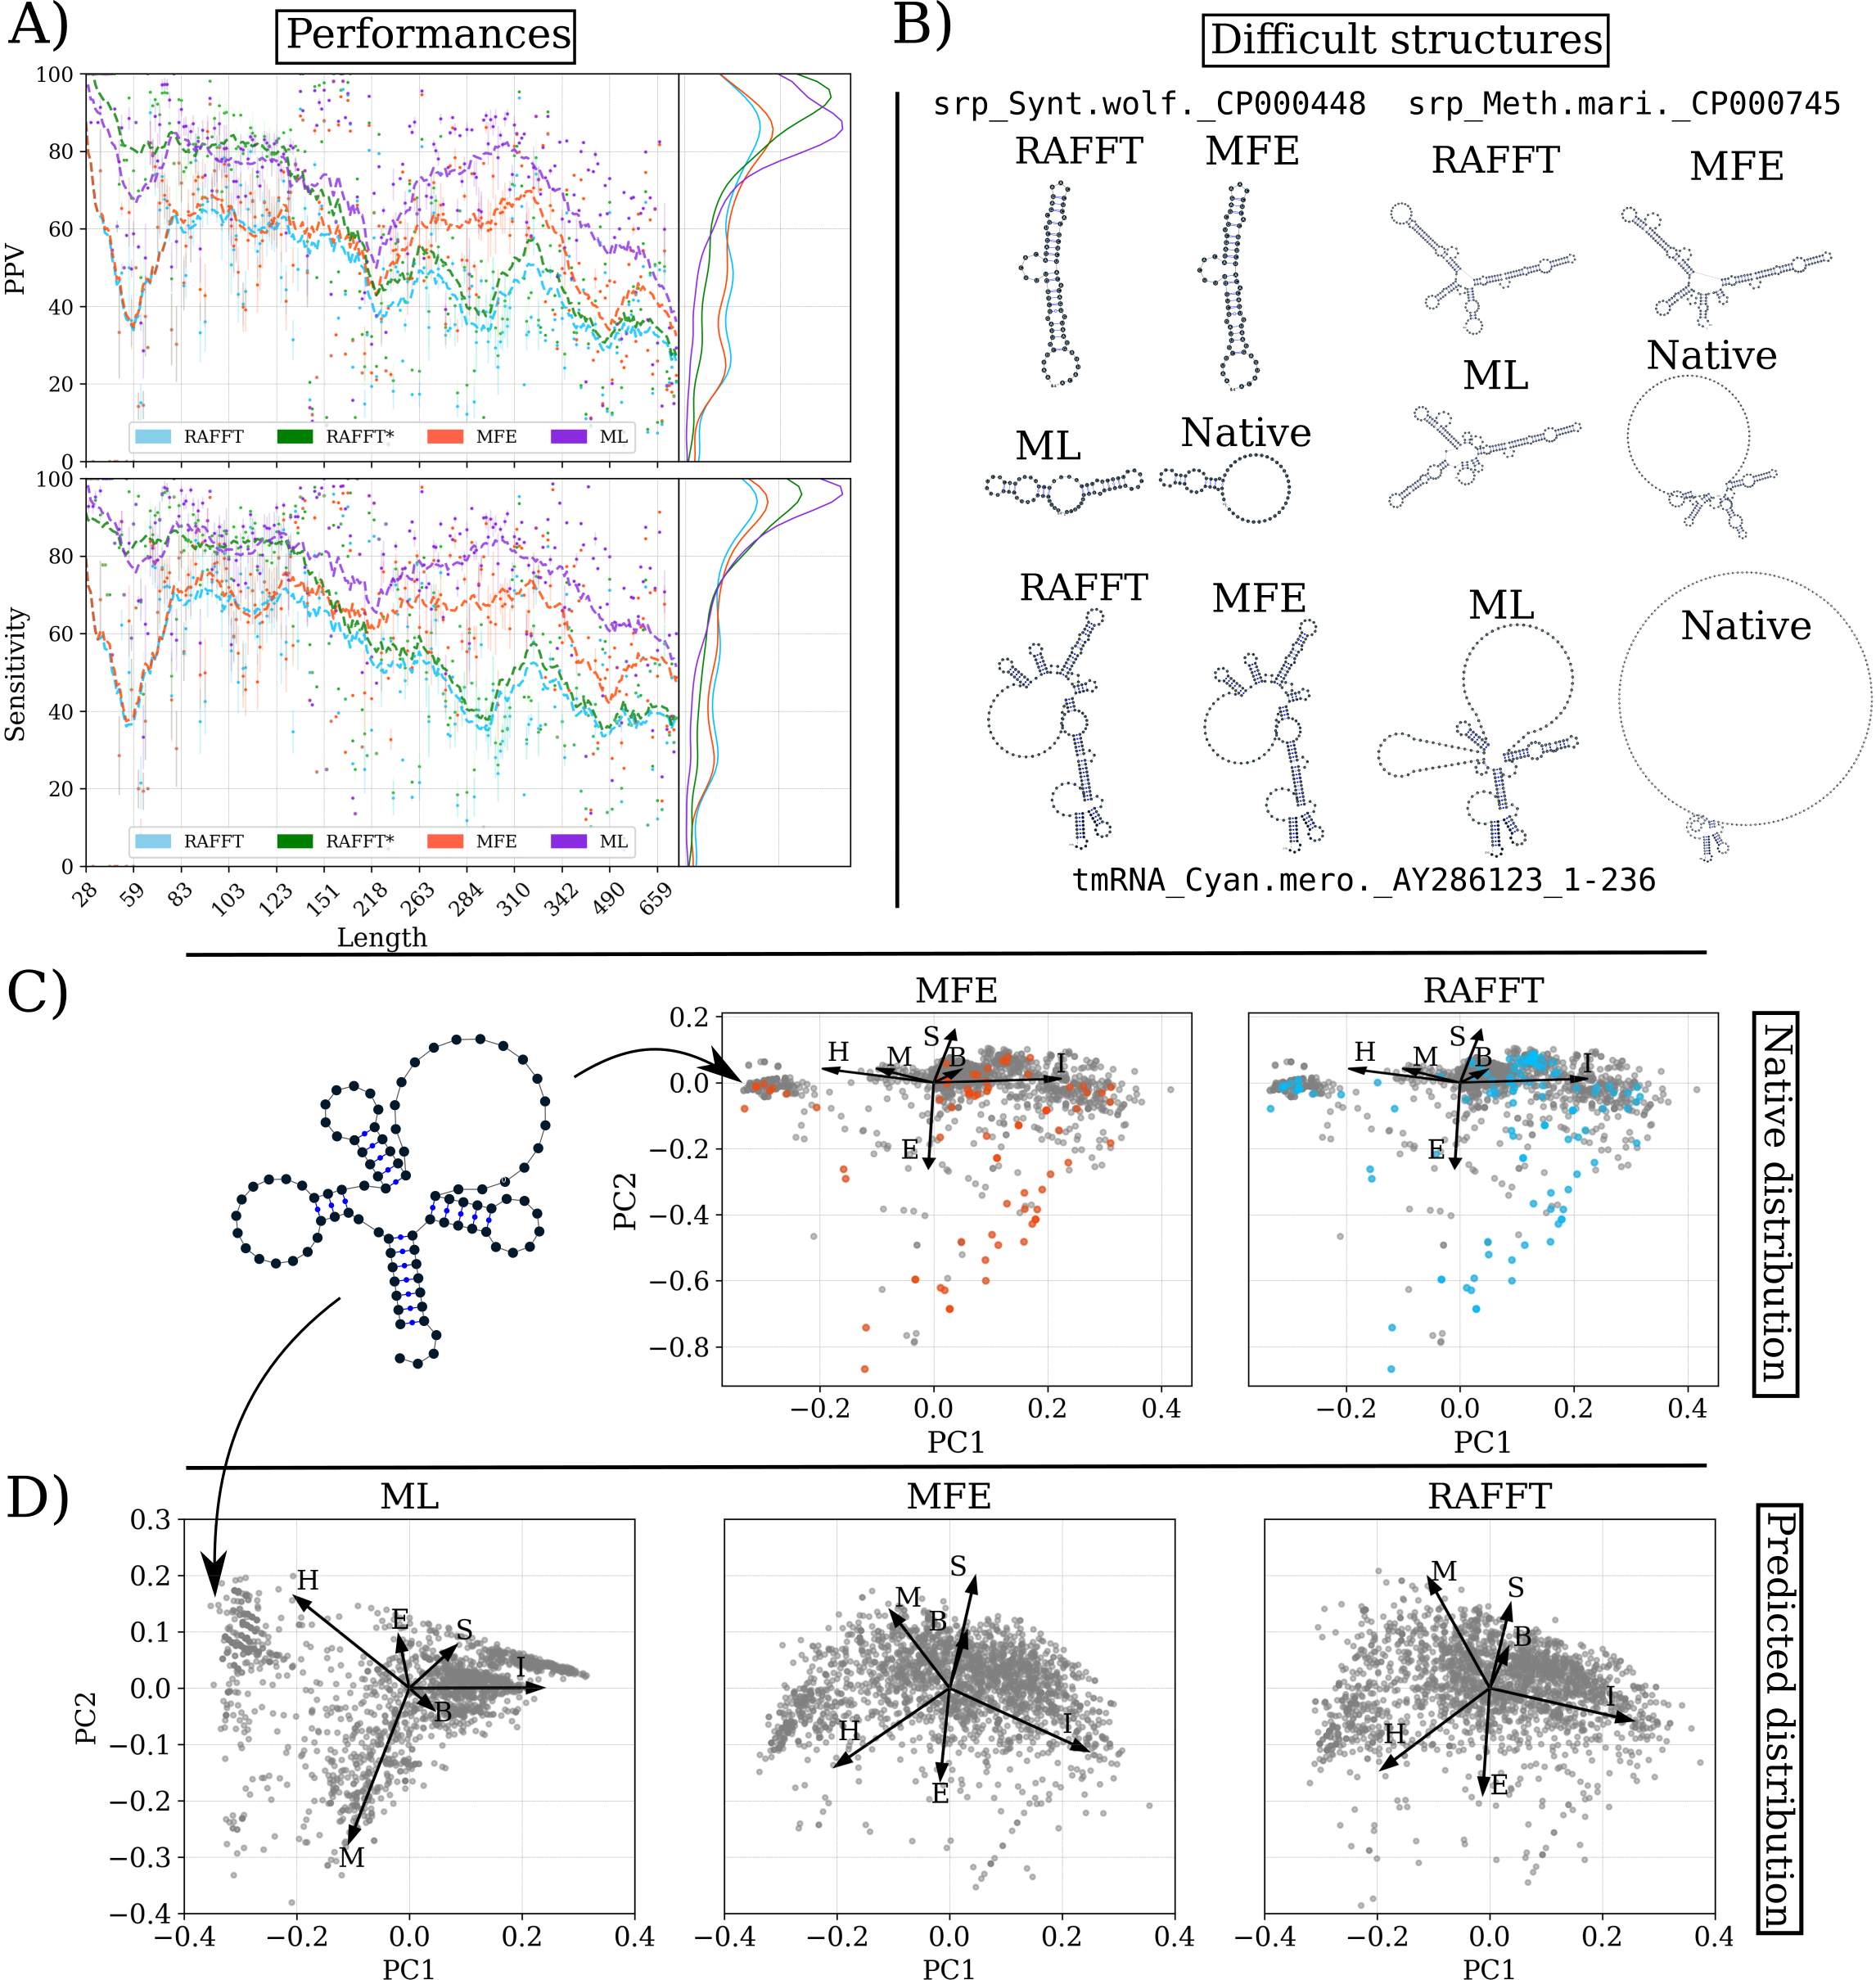
\includegraphics[width=.9\linewidth]{../res/images/rafft/perf_illed.png}
	\caption{\label{perf_fig} \textbf{\texttt{RAFFT}'s performance on folding task.} (A) PPV and sensitivity \emph{vs} sequence length. In the left panels, \texttt{RAFFT} (in blue) shows the scores when for the structure (out of $N=50$ predictions) with the lowest free energy, whereas \texttt{RAFFT}* (in green) shows the best PPV score in that ensemble. Each dot corresponds to the mean performance for a given sequence length, and vertical lines display their standard deviation. The right panels of both figures show the distribution of PPV and sensitivity sequence-wise. (B) List of structures that are challenging to predict using the thermodynamic model. The sequence names are from the dataset. The native structures have large regions with unpaired nucleotides. (C) PCA for structures in the dataset. An example of structures with a large hairpin (\textbf{H}) is shown on the left. The points marked in orange (resp. blue) are the MFE (resp. \texttt{RAFFT}) structures with PPV \(\leq\) \(10\%\). (D) PCA for the predicted structures. The MFE and \texttt{RAFFT} structure spaces look similar and more diverse than the ML structure space, closer to the native structure space.}
\end{figure*}

\section*{Results}
\subsection*{Application to the folding task}
We started by analyzing the prediction performances with respect to sequence lengths: we averaged the performances at fixed sequence length. Figure \ref{perf_fig}A shows the performance in predicted positive values (PPV) and sensitivity for the three methods. It shows that the ML method consistently outperformed \texttt{RAFFT} and MFE predictions. The $t$-test between the ML and the MFE predictions revealed not only a significant difference (p-value \(\approx\) $10$\textsuperscript{$-12$}) but also a substantial improvement of $14.5\%$ in PPV. \texttt{RAFFT} showed performances similar to the MFE predictions; however, \texttt{RAFFT} is significantly less accurate ($p$-value \(\approx\) $0.0002$), with a drastic loss of performance for sequences of length greater than $300$ nucleotides. In contrast, when only the most accurate predicted structure among the $50$ recorded structures per sequence was considered, we obtained $57.9\%$ of PPV and $63.2\%$ of sensitivity on average. The gain of performance was even more substantial for sequences of length below $200$ nucleotides. The PPV was $79.4\%$, and the sensitivity was $81.2\%$. In contrast, longer sequences did not display any gain. The average performances are shown in table \ref{average_perf}. We also investigated the relation to the number of bases between paired bases (base pair spanning), but we found no striking effect, as already pointed out in one previous study \cite{amman13_troub_long_range_base_pairs_rna_foldin}.

All methods performed poorly on two groups of sequences: one group of $80$ nucleotides long RNAs, and the second group of around $200$ nucleotides. Figure \ref{perf_fig}B shows three examples of such sequences. Both groups have large unpaired regions, which for the first group lead to structures with average free energies $9.8\ \textrm{kcal/mol}$ according to our dataset. The PCA analysis of the native structure space, shown in Figure \ref{perf_fig}C, reveals a propensity for interior loops and the presence of large unpaired regions like hairpins or external loops. Figure \ref{perf_fig}D shows the structure space produced by the ML predictions, which seems close to the native structure space. In contrast, the structure spaces produced by \texttt{RAFFT} and \texttt{RNAfold} (MFE) are similar and more diverse.

\begin{figure*}[t!]
	\centering
	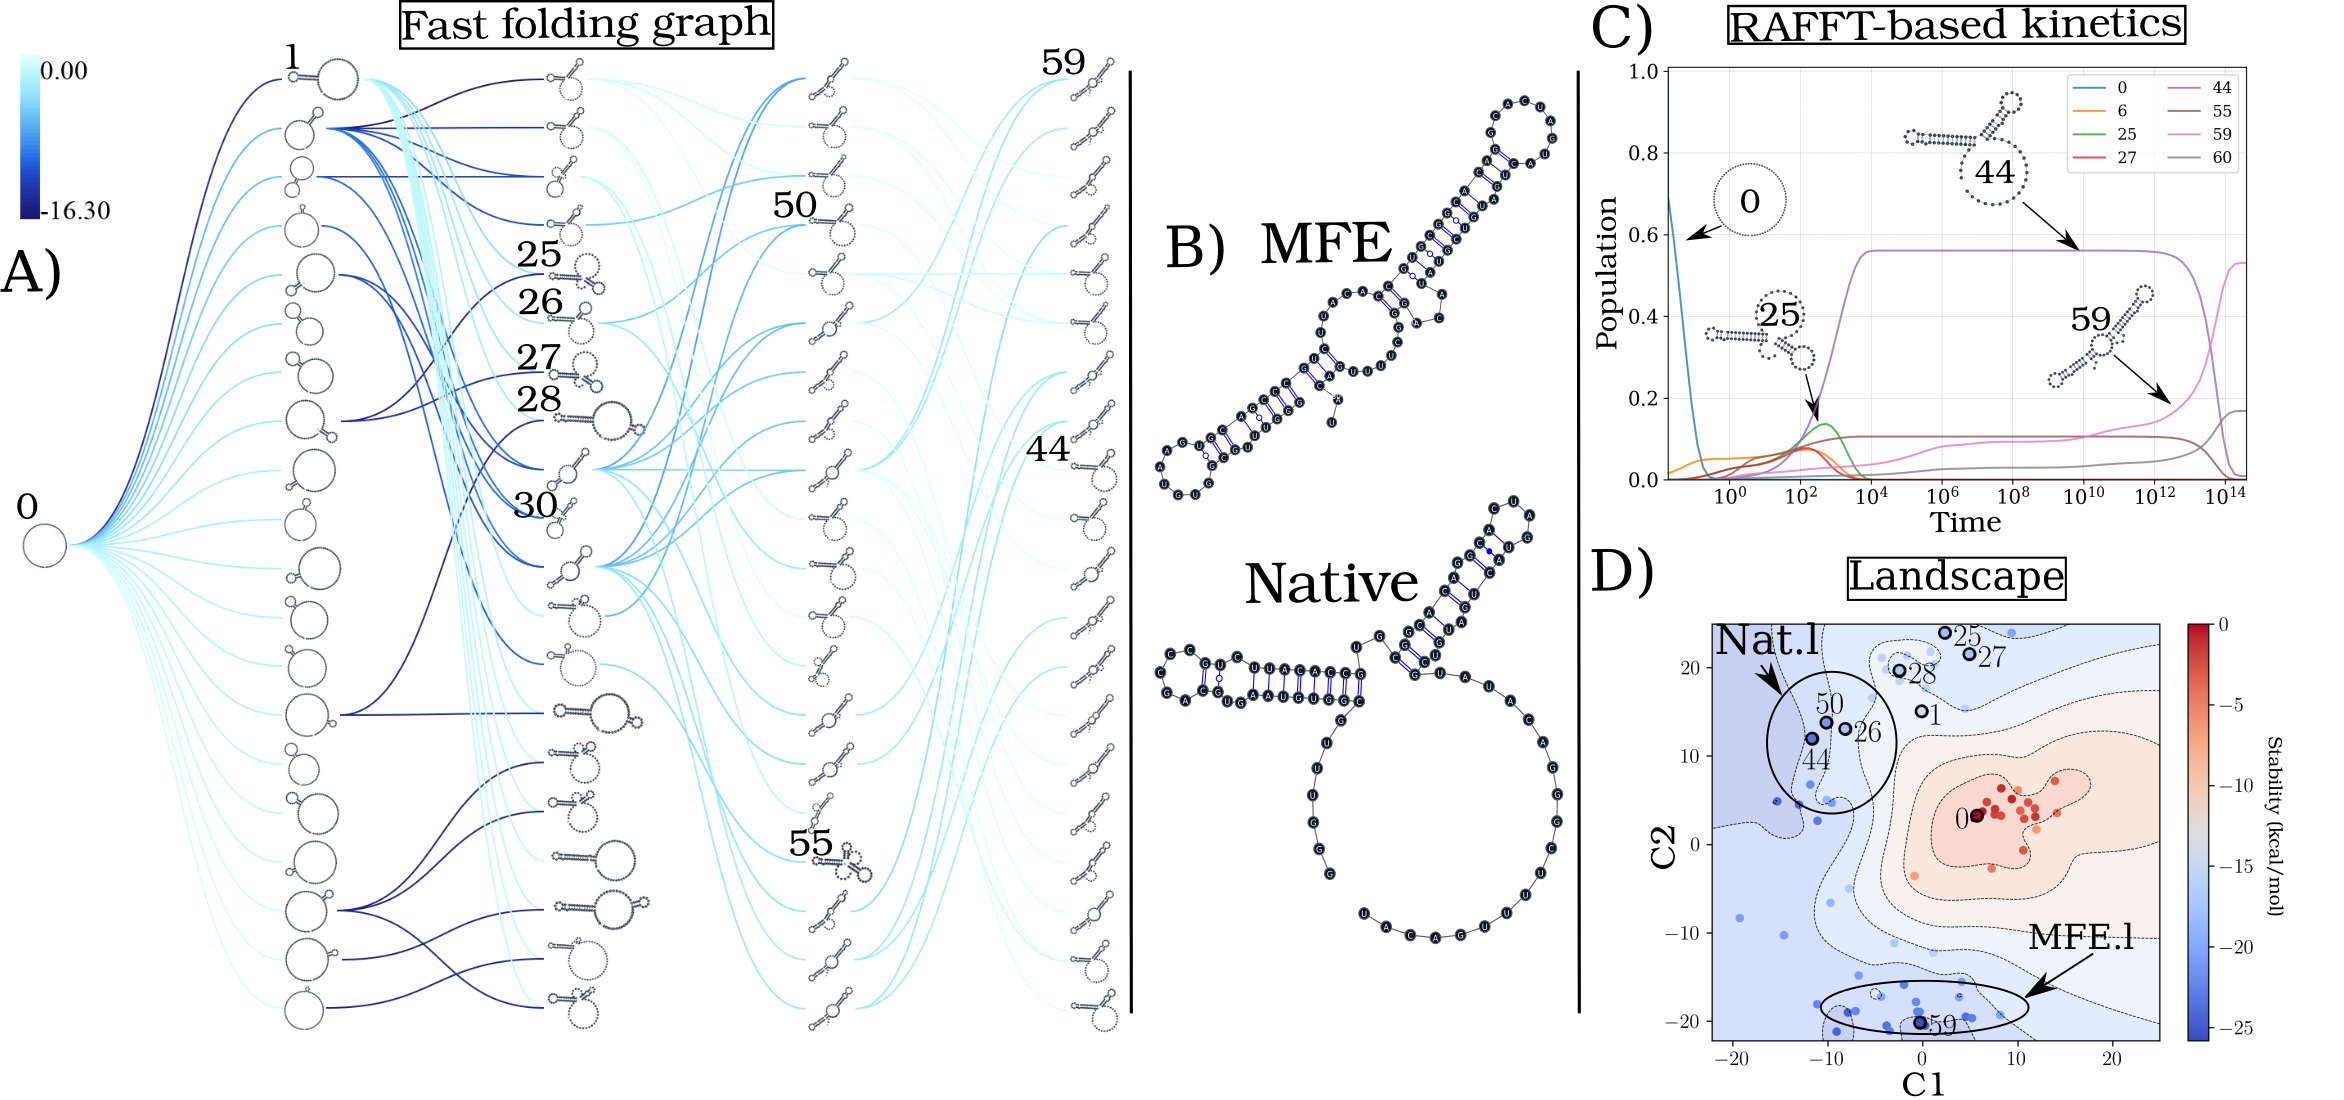
\includegraphics[width=0.9\linewidth]{../res/images/rafft/test_case.png}
	\caption{\label{test_case}\textbf{Application of the folding kinetic ansatz on CFSE.}  (A) Fast-folding graph in four steps and $N=20$ structures stored in a stack at each step. The edges are coloured according to \(\Delta \Delta G\). At each step, the structures are ordered by their free energy from top to bottom. The minimum free energy structure found is at the top left of the graph. A unique ID annotates visited structures in the kinetics. For example, ``$59$" is the ID of the MFE structure. (B) MFE (computed with \texttt{RNAfold}) and the native CFSE structure. (C)The change in structure frequencies over time. The simulation starts with the whole population in the open-chain or unfolded structure (ID 0). The native structure (\textbf{Nat.l}) is trapped for a long time before the MFE structure (\textbf{MFE.l}) takes over the population. (D) Folding landscape derived from the $68$ distinct structures predicted using \texttt{RAFFT}. The axes are the components optimized by the MDS algorithm, so the base pair distances are mostly preserved. Observed structures are also annotated using the unique ID. MFE-like structures (\textbf{MFE.l}) are at the bottom of the figure, while native-like (\textbf{Nat.l}) are at the top.}
\end{figure*}
\subsection*{Selected applications of the kinetic ansatz}
We started with the CFSE, a natural RNA sequence of $82$ nucleotides with a structure determined by sequence analysis and obtained from the RFAM database. This structure has a pseudoknot which is not taken into account here.

Figures \ref{test_case}A and \ref{test_case}B show respectively the fast-folding graph constructed using \texttt{RAFFT}, and the MFE and native structures for the CFSE. The fast-folding graph is computed in four steps. At each step, stems are constructed by searching for $n=100$ positional lags and, a set of $N=20$ structures (selected according to their free energies) are stored in a stack. The resulting fast-folding graph consists of $68$ distinct structures, each of which is labelled by a number. Among the structures in the graph, $6$ were found similar to the native structure ($16/19$ base pairs differences). The structure labelled ``$29$'' in the graph leading to the MFE structure ``$59$'' is the $9^{th}$ in the second stack. When storing less than $9$ structures in the stack at each step, we cannot obtain the MFE structure using \texttt{RAFFT}; this is a direct consequence of the greediness of the proposed method. To visualize the energy landscape drawn by \texttt{RAFFT}, we arranged the structures in the fast-folding graph onto a surface according to their base-pair distances; for this we used the multidimensional scaling algorithm implemented in the \texttt{scipy} package.  Figure \ref{test_case}D shows the landscape interpolated with all the structures found; this landscape illustrates the bi-stability of the CFSE, where the native and MFE structures are in distinct regions of the structure space.

From the fast-folding graph produced using \texttt{RAFFT}, the transition rates from one structure in the graph to another are computed using the formula given in Eq \ref{Eq:metropolis}. Starting from a population of unfolded structure and using the computed transition rates, the native of structures is calculated using Eq \ref{Eq:kenetics}. Figure \ref{test_case}C shows the frequency of each structure; as the frequency of the unfolded structure decreases to $0$, the frequency of other structures increases. Gradually, the structure labelled ``$44$", which represents the CFSE native structure, takes over the population and gets trapped for a long time, before the MFE structure (labelled "$59$") eventually becomes dominant. Even though the fast-folding graph does not allow computing energy landscape properties (saddle, basin, etc.), the kinetics built on it reveals a high barrier separating the two meta-stable structures (MFE and native). 

\begin{figure*}[t!]
	\centering
	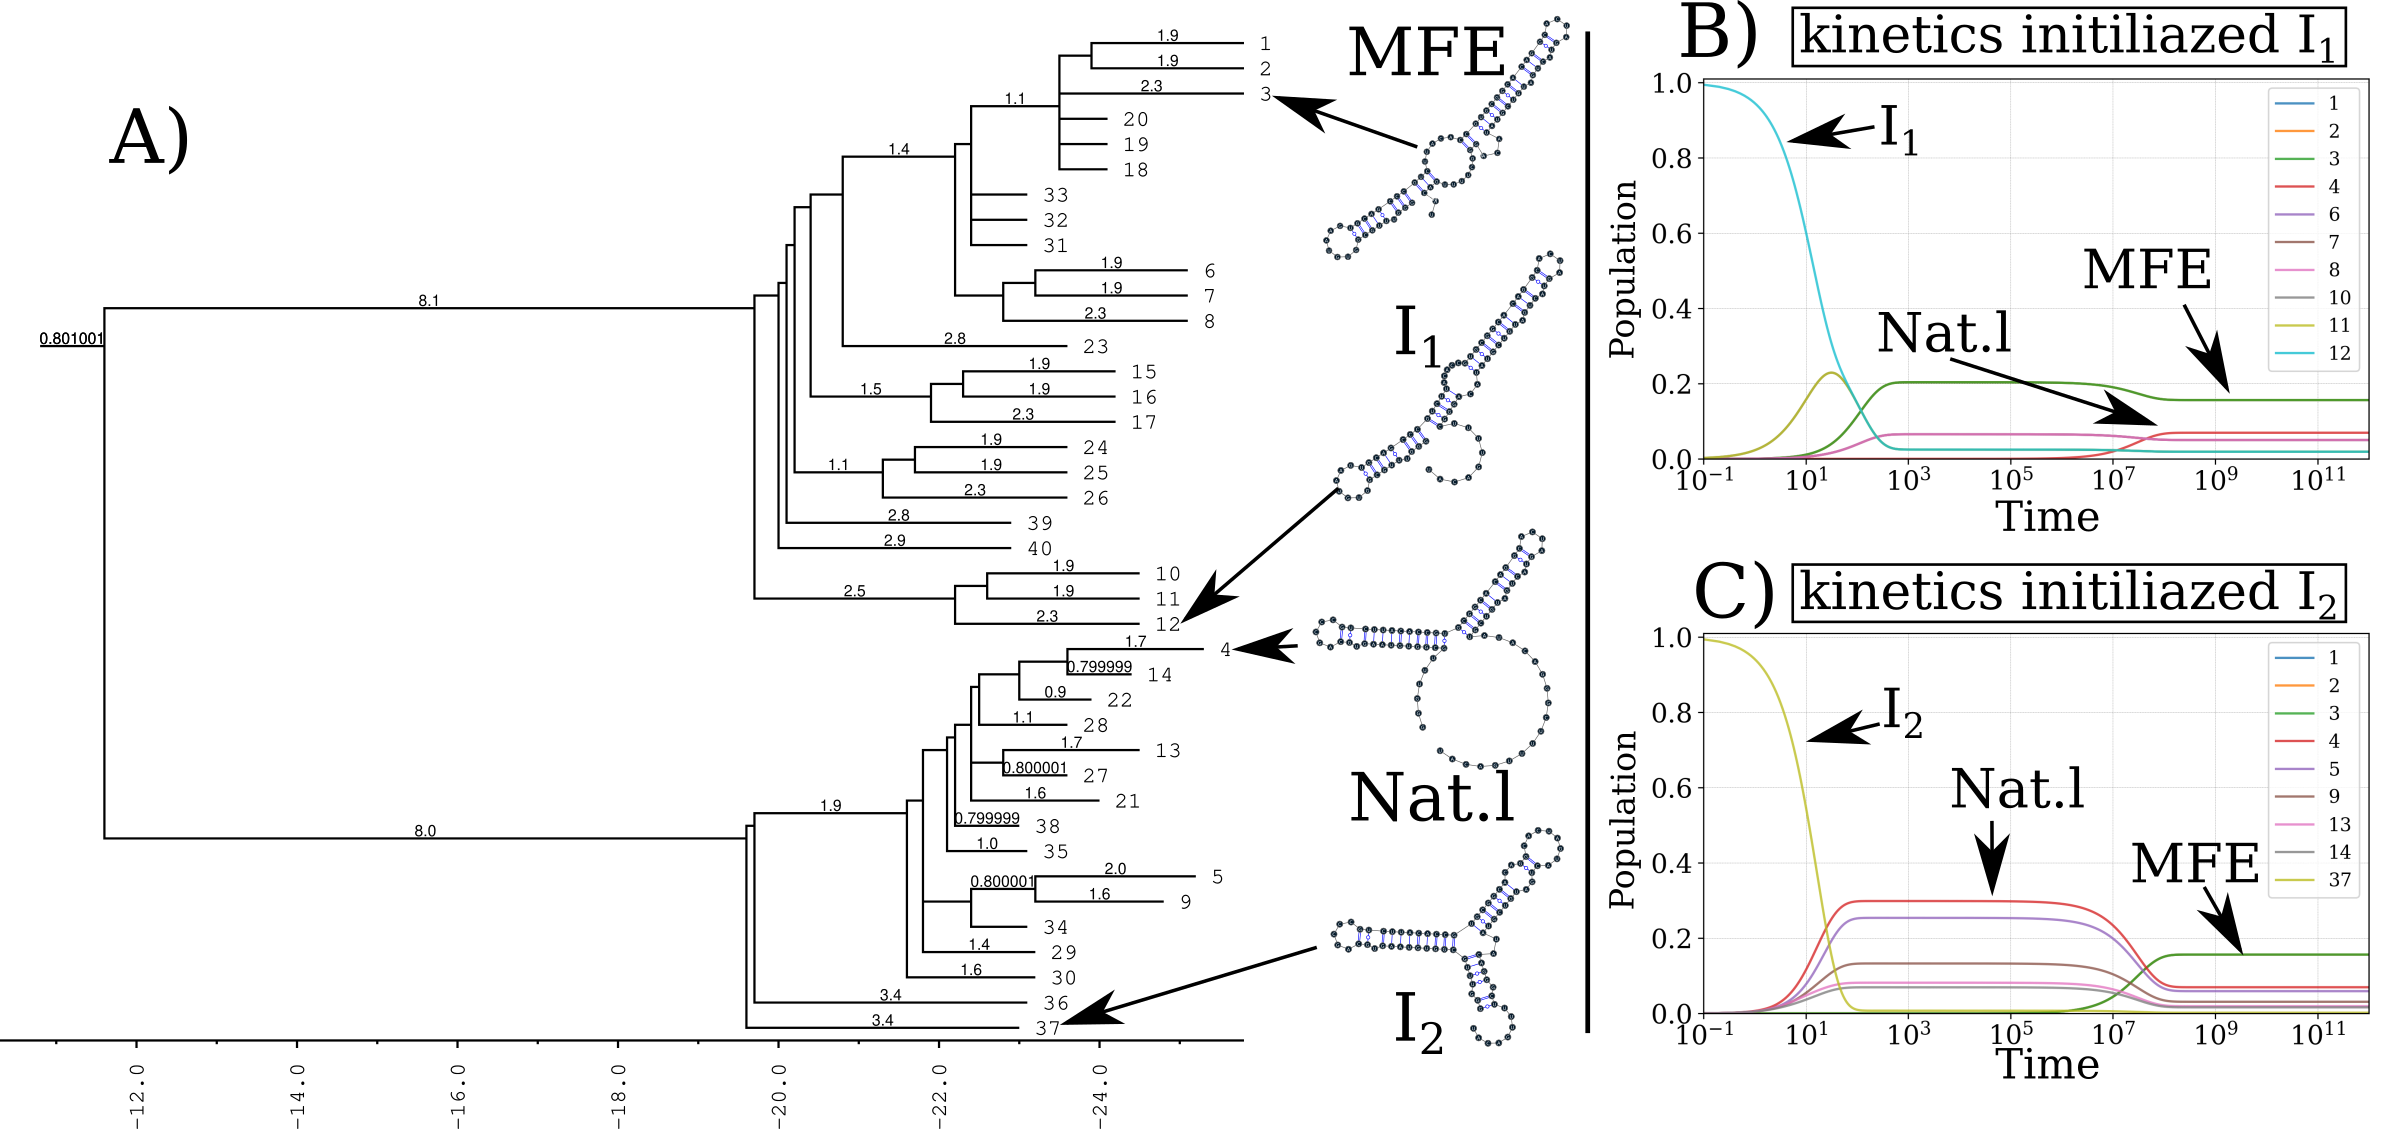
\includegraphics[width=0.9\linewidth]{../res/images/rafft/kinetic_treekin.png}
	\caption{\label{treekin}\textbf{Folding kinetics of CFSE using \texttt{Treekin}. }A) Barrier tree of the CFSE. From a set of $1.5\times10^6$ sub-optimal structures, $40$ local minima were found,  connected through saddle points. The tree shows two alternative structures separated by a high barrier with the global minimum (MFE structure) on the right side. (B) Folding kinetics with initial population $I_1$. Starting from an initial population of $I_1$, as the initial frequency  decreases, the others increase, and gradually the MFE structure is the only one populated.  (C) Folding kinetics with initial population $I_2$. When starting with a population of $I_2$, the native structure (labelled \textbf{Nat.1} ) is observable, and gets kinetically trapped for a long time due to the high energy barrier separating it from the MFE structure.}
\end{figure*}

Our kinetic simulation was then compared to \texttt{Treekin} \cite{flamm02_barrier_trees_degen_lands}. First, we generated \(1.5 \times 10^6\) sub-optimal structures up to $15 \ \textrm{kcal/mol}$ above the MFE structure using \texttt{RNAsubopt} \cite{lorenz11_vienn_packag}. Since the MFE is $\Delta G_s=-25.8 \ \textrm{kcal/mol}$, the unfolded structure could not be sampled. Second, the ensemble of structures is coarse-grained into $40$ competing basins using the tool \texttt{barriers} \cite{flamm02_barrier_trees_degen_lands}, with the connectivity between basins represented as a barrier tree (see Figure \ref{treekin}A). When using \texttt{Treekin}, the choice of the initial population is not straightforward. Therefore we resorted to two initial structures $I_1$ and $I_2$ (see Figure \ref{treekin}B and \ref{treekin}C, respectively). In Figure \ref{treekin}B, the trajectories show that only the kinetics initialized in the structure $I_2$ can capture the complete folding dynamics of CFSE, in which the two metastable structures are visible. Thus, in order to produce a folding kinetics in which the native and the MFE structures are visible, the kinetic simulation performed using \texttt{Treekin} required a particular initial condition and a barrier tree representation of the energy landscape built from a set of  $1.5 \times 10^6$ structures. By contrast, using the fast-folding graph produced by \texttt{RAFFT}, which consists only of $68$ distinct structures, our kinetic simulation produces complete folding dynamics starting from a population of unfolded structure.

As a second illustrative example, we applied both kinetic models to the classic bi-stable sequence \texttt{GGCCCCUUUGGGGGCCAGACCCCUAAAGGGGUC}. For \texttt{Treekin}, we first sampled the whole space of \(20 \times 10^3\) sub-optimal structures from the unfolded state to the MFE structure, and from that set, $40$ basins were also computed using \texttt{barriers}. The barrier tree in Figure \ref{class_examp} shows the bi-stable landscape, where the two deepest minima are denoted $S_A$ and $S_B$. As in the first application, we also chose two initializations with the structures denoted $I_1$ and $I_2$ in Figure \ref{class_examp}A and \ref{class_examp}B. Secondly, we simulate the kinetics starting from the two initial conditions (See Figure \ref{class_examp}B). When starting from $I_2$, the slow-folding dynamics is visible:  $S_B$ first gets kinetically trapped, and the MFE structure ($S_A$) only takes over later on. For our kinetic ansatz, we started by constructing the fast-folding graph using \texttt{RAFFT}, consisting of only $46$ distinct structures. The resulting kinetics, shown in Figure \ref{class_examp}B' was found qualitatively close to the barrier kinetics initialized with structure $I_2$. Once again, with few as $48$ structures, our proposed kinetic ansatz can produce complete folding dynamics starting from a population of unfolded structure.

\begin{figure*}[t!]
	\centering
	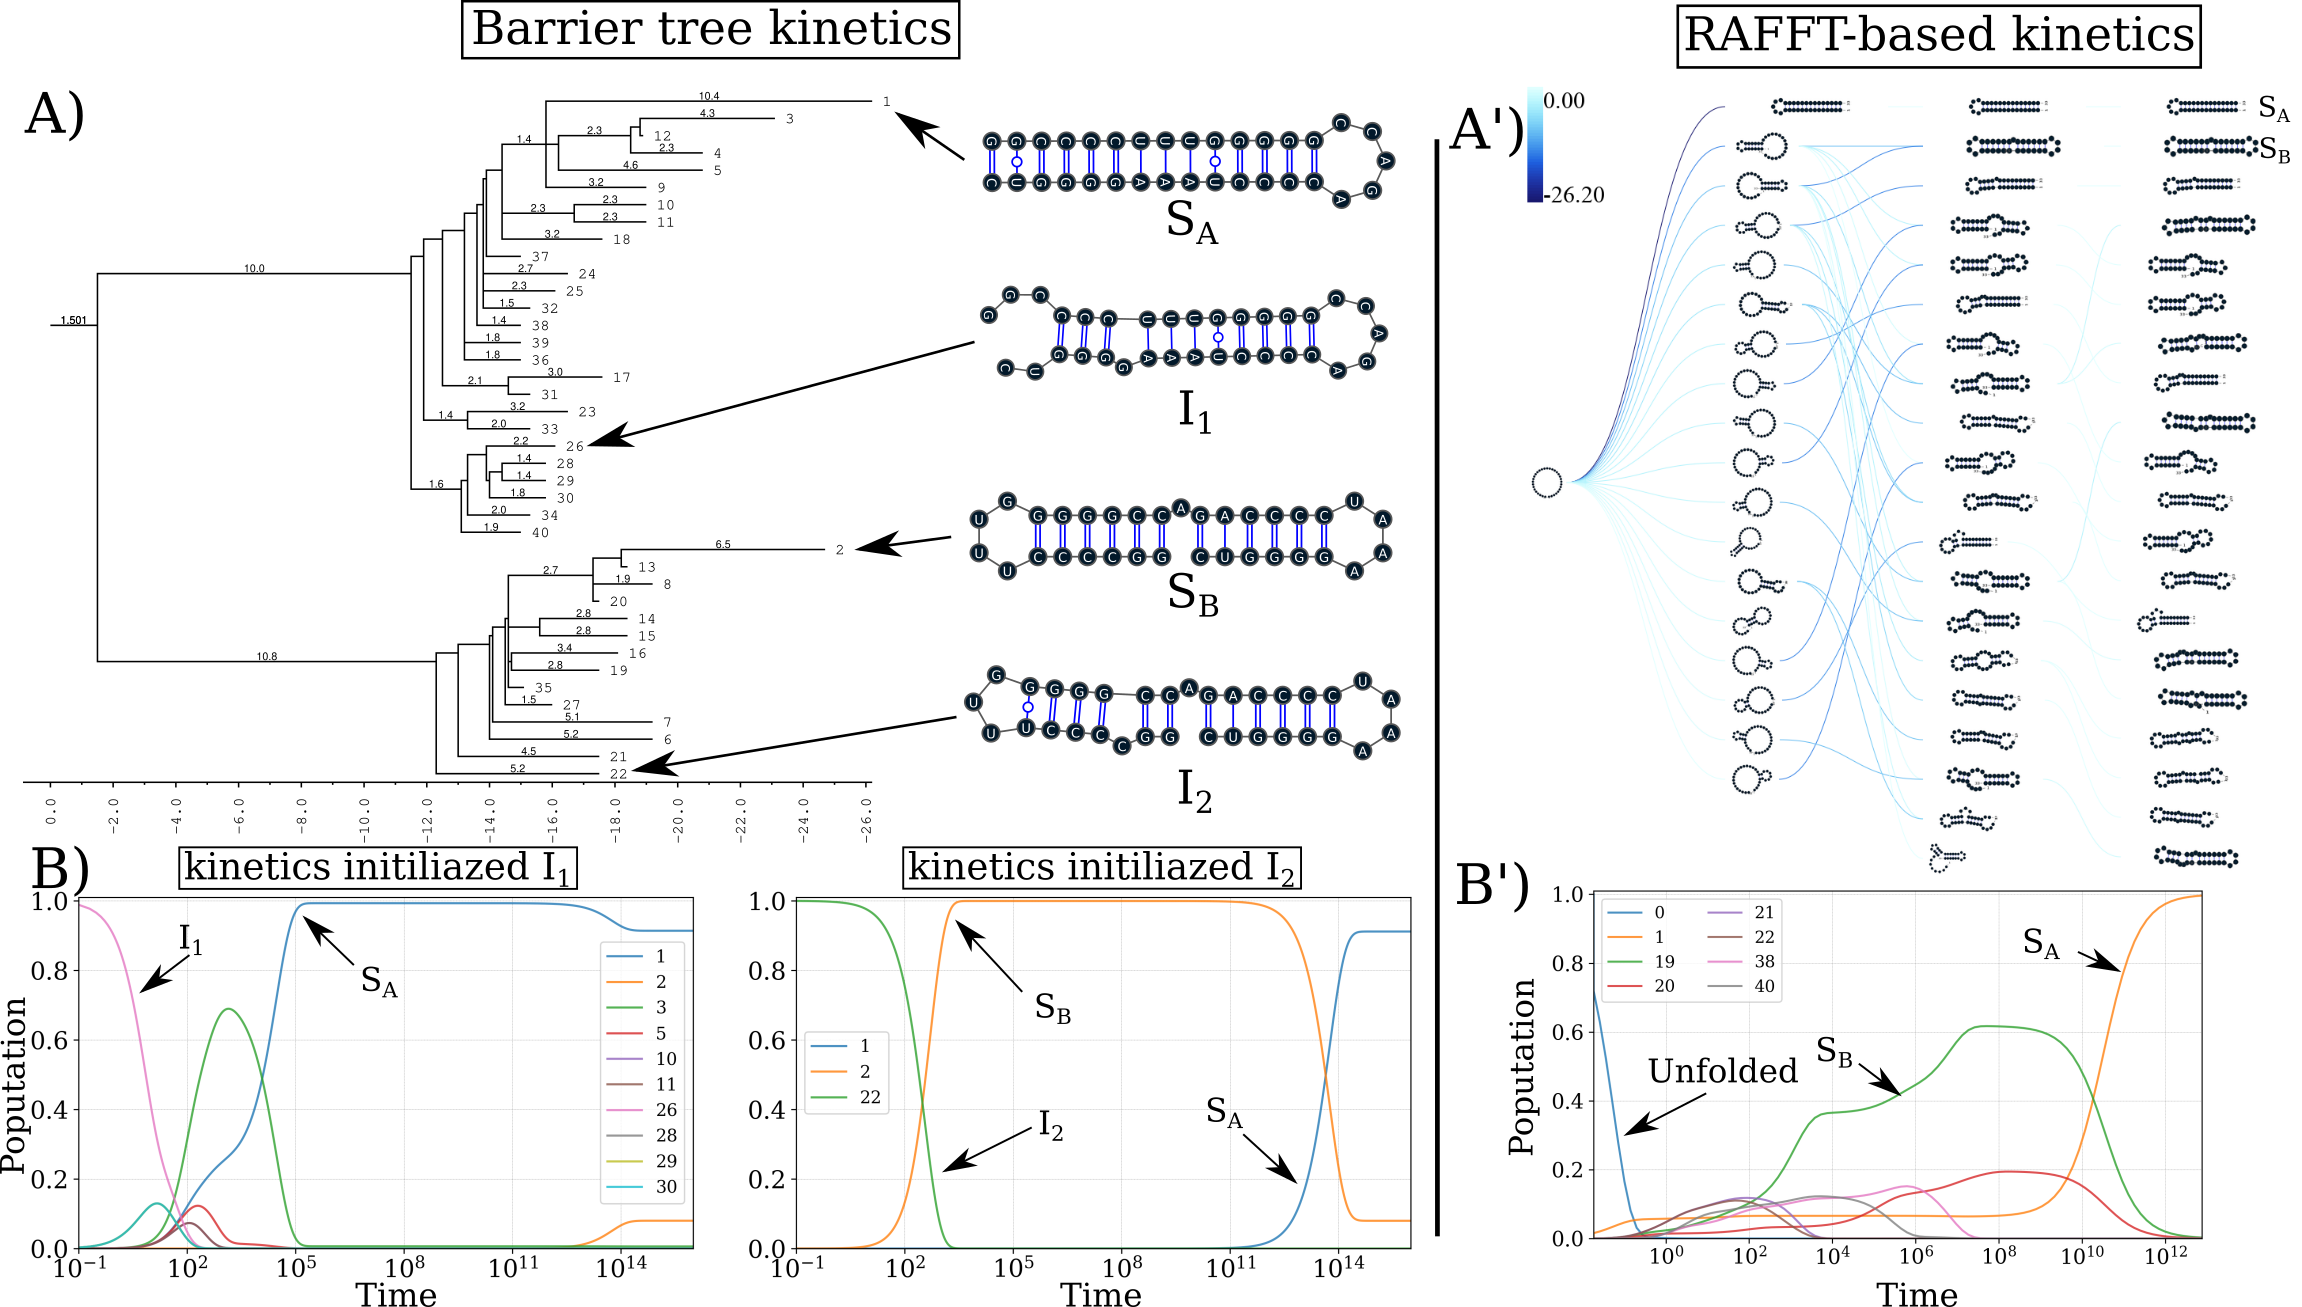
\includegraphics[width=0.9\linewidth]{../res/images/rafft/kine_bi_sta.png}
	\caption{\label{class_examp}\textbf{\texttt{RAFFT} \emph{vs} \texttt{Treekin}: folding kinetics of a bi-stable RNA sequence.} (A) Barrier tree for the bi-stable example sequence. The local minima and the corresponding barriers are computed from the complete enumeration of the structure space. The bi-stability is visible on the barrier tree through the two branches separated by a high barrier.  (B) Folding kinetics trajectories. The left plot shows the folding dynamics starting from a population with $I_1$, and the right size is the kinetics when the population is initialized in structure $I_2$. When starting from $I_1$, $S_A$ is quickly populated; starting from $I_2$, the bi-stability is more apparent.  (A') Fast-folding graph using \texttt{RAFFT}. A maximum of $N=20$ structures are stored in a stack at each step and overall $46$ distinct structures are visited. (B') Folding kinetics trajectory obtained from the fast-folding graph (indices are different from the barrier tree indices). The dynamics starts with a population with only unfolded structure, and slowly, $S_B$ is populated and gets trapped for a long time before the MFE structure $S_A$ becomes populated.}
\end{figure*}

\section*{Discussion}
We have proposed a method for RNA structure and dynamics predictions called \texttt{RAFFT}. Our method was inspired by the experimental observation of parallel fast-folding pathways. We designed an algorithm that produces parallel folding pathways, in which stems are formed sequentially, to mimic this observation. Then, to model the slow part of the folding process, we proposed a kinetic ansatz that exploits the parallel fast-folding pathways predicted.

First, we compared the algorithm performance for the folding task. Two structure estimates were compared with our method: the MFE structure computed using \texttt{RNAfold}, and the ML estimate using \texttt{MxFold2}. Other thermodynamic-based and ML-based tools were investigated but not shown here because their performances were found to be very similar to the one of \texttt{MxFold2} and \texttt{RNAfold} (See SI for the complete benchmark). When we considered the lowest energy structure, the comparison of \texttt{RAFFT} to existing tools confirmed the overall validity of our approach. In more detail, comparison with thermodynamic/ML models yielded the following results. First, the ML predictions performed consistently better than both \texttt{RAFFT} and the MFE approaches, where the PPV $=70.4\%$ and sensitivity $=77.1\%$ on average. Second, the ML methods produced loops, such as long hairpins or external loops. We argue that the density of those loops correlate with the ones in the benchmark dataset, which a PCA analysis revealed too. In contrast, the density of loops was lower in the structure spaces produced by \texttt{RAFFT} and MFE, implying some over-fitting in the ML model. Finally, known structures obtained through covariation analysis reflect structures \textit{in vivo} conditions. Therefore, the structures predicted by ML methods may not only result from their sequences alone but also from their molecular environment, e.g. chaperones. We expect the thermodynamic methods to provide a more robust framework for the study of sequence-to-structure relations.

With respect to MFE-based tools, we obtained a substantial gain of performance when analyzing \(N=50\) predicted structures per sequence and not only the lowest energy one. This gain was even more remarkable for sequences with fewer than $200$ nucleotides, reaching the accuracy of ML predictions. So how does \texttt{RAFFT} produce better structures, although these structures are less thermodynamically stable? The interplay of three effects may explain this finding. First, the MFE structure may not be relevant because active structures can be in kinetic traps. Second, \texttt{RAFFT} forms a set of pathways that cover the free energy landscape until they reach local minima, yielding multiple long-lived structures accessible from the unfolded state. Third, the energy function is not perfect, so that the MFE structures computed by minimizing it may not in fact be the most stable. 

We also showed that the fast-folding graph produced by \texttt{RAFFT} can be used to reproduce state-of-the-art kinetics, at least qualitatively. Our method demonstrated three main benefits. First, the kinetics can be drawn from as few as $68$ structures, whereas the barrier tree may require millions. Second, the kinetics ansatz describes the complete folding mechanism starting from the unfolded state. Third, for the length range tested here, the procedure did not require any additional coarse-graining into basins. (Longer RNAs might require such a coarse-graining step, in which structures connected in the fast-folding graph are merged together).

Based on our results, we believe that the proposed method is a robust heuristic for structure prediction and folding dynamics. The folding landscape depicted by \texttt{RAFFT} was designed to follow the kinetic partitioning mechanism, where multiple folding pathways span the folding landscape. This approach has shown good predictive potential. Furthermore, we derived a kinetic ansatz from the fast-folding graph to model the slow part of the folding dynamics. It was shown to approximate the usual kinetics framework qualitatively, albeit using many fewer structures. 

However, further improvements and extensions of the algorithm may be investigated. For starters, the choice of stems is limited to the largest in each positional lag, a greedy choice which may not be optimal. Furthermore, we have constructed parallel pathways leading to a diversity of accessible structures, but we have not given any thermodynamic-based criterion to identify which are more likely to resemble the native structure. We suggest using an ML-optimized score to this effect. Our method can also find applications in RNA design, where the design procedure could start with the identification of long-lived intermediates and use them as target structures. We also believe that mirror encoding can be helpful in phylogenetic analysis. Indeed, the correlation spectra \(\text{cor}(k)\) computed here contained global information of base-pairing that can be used as a similarity measure.



%\section*{Conclusions}

\section*{Data availability}
The implementation in \texttt{python3.0} of \texttt{RAFFT} and the benchmark data used in this manuscript are available at \url{https://github.com/strevol-mpi-mis/RAFFT}. We also provide the scripts used for the figures and kinetic analyses.